%%%%%%%%%%%%%%%%%%%%%%%%%%%%%%%%%%%%%%%%%%%%%%%%%%%%%%%%%%%%%%%%%%%%%%%%%%%%%%%
%%%%%%%%%%%%%%%%%%%%%%%%%%%%%%%%%%%%%%%%%%%%%%%%%%%%%%%%%%%%%%%%%%%%%%%%%%%%%%%
%%%%%%%%%%%%%%%%%%%%%%%%%%%%%%%%%%%%%%%%%%%%%%%%%%%%%%%%%%%%%%%%%%%%%%%%%%%%%%%
%
\begin{figure}[h]
\centering
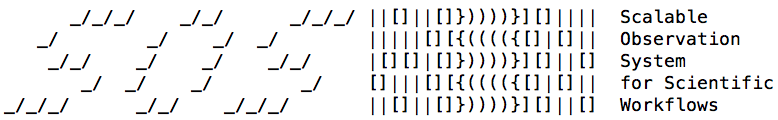
\includegraphics[width=\columnwidth]{images/sosflow_masthead.png}
\label{fig_masthead}
\end{figure}
%
%%%%%%%%%%%%%%%%%%%%%%%%%%%%%%%%%%%%%%%%%%%%%%%%%%%%%%%%%%%%%%%%%%%%%%%%%%%%%%%
%%%%%%%%%%%%%%%%%%%%%%%%%%%%%%%%%%%%%%%%%%%%%%%%%%%%%%%%%%%%%%%%%%%%%%%%%%%%%%%
\section{Introduction}
%

%
%
\subsection{The Scalable Observation System} %-----------------------------%
%
SOSflow can be used for a variety of
purposes:
\begin{itemize}
    \item Aggregation of performance data at runtime
    \item Providing holistic views of multi-component
        distributed scientific workflows
    \item Coordinating in situ operations with global
        analytics
    \item Synthesizing application and system metrics
        with scientific data for deeper performance
        understanding
    \item Extending the functionality of existing HPC
        codes
    \item Resource management, load balancing, online
        performance tuning, and much more...
\end{itemize}
%
There are many more ways to use the SOSflow platform than the scope of this
paper can contain.
%
\begin{figure}[h]
\centering

\includegraphics[width=\columnwidth]{images/placeholder.jpg}
\caption{An overview of the SOS model.}
\label{fig_sos_overview}
\end{figure}
%
This paper is principally concerned with describing the architecture and use
of SOSflow, and concludes with a set of representative experiments.
%
The experiments selected here are abstract, though they were performed on
real-world HPC machines.
%
This choice was deliberate, to encourage the reader to imagine how SOSflow
could facilitate their own use cases, rather than the reader seeing it as
addressing a specific case that is not of interest to them.
%
%%%%%%%%%%%%%%%%%%%%%%%%%%%%%%%%%%%%%%%%%%%%%%%%%%%%%%%%%%%%%%%%%%%%%%%%%%%%%%%
%%%%%%%%%%%%%%%%%%%%%%%%%%%%%%%%%%%%%%%%%%%%%%%%%%%%%%%%%%%%%%%%%%%%%%%%%%%%%%%
%%%
%%%  EOF
%%%

